\section{Designs}
Now that all the different components have been described, it's time to construct some designs they can be used with.

\subsection{Potential Divider}
One of the more simple, yet incredibly important, designs is the potential divider.
This circuit consists of two or more resistors connected up in series.
A voltage can then be measured between each resistor.
This voltage will be proportional to the values of the resistances and the power supply voltage.

\begin{enumerate}
\item Please take two $10K\Omega$ resistors and connect them up as shown
\item Turn on the power supply
\item Use the digital multimeter to measure the voltage at the midpoint
\item Replace R? with a resistor of value $5K\Omega$
\item Measure the voltage at the midpoint
\item Replace R? with a resistor of value $20K\Omega$
\item Measure the voltage at the midpoint
\item What would happen if you replaced R? with a resistor of value $30K\Omega$?
\item Check if you're correct
\end{enumerate}

There is a device known as a \emph{potentiometer}, or \emph{pot.}, which consists of a long track of resistive material with a metal contact in the middle.
This device makes it easy to create a potential divider, by connecting the ends of the track up to the power supply and then adjusting the contact to the appropriate position.

\subsection{Filters}
Filters are useful circuits which allow particular signals to be subtracted from the input signal.
A \emph{high pass} filter is one which removes low frequencies from a signal, whereas a \emph{low pass} filter can be used to remove high frequecies from the signal.
These can be combined to only allow a small set of frequencies through.

You will now construct a high pass and a low pass filter, and see how they work.

\begin{enumerate}
\item Construct the filter circuit as shown
\item \label{enum:des:filter:setfreq}Set the signal generator to 10Hz
\item Use the oscilloscope probe to observe the output of the signal generator
\item Use the oscilloscope probe to observe the output of the filter
\item \label{enum:des:filter:noteamp}Note any change in the signals amplitude
\item Repeat steps \ref{enum:des:filter:setfreq} through \ref{enum:des:filter:noteamp} for 50Hz, 100Hz, 150Hz, 200Hz, and 250Hz
\item What would happen at 1KHz?
\item Check if you're correct
\end{enumerate}

\subsection{Op-Amp}
There are many different circuits that the operational amplifier can be used in.
Today we will briefly look at some of the simpler ones.

\subsubsection{Comparator}
The differential inputs of the op-amp, and its high gain, means it can be used to detect which of two signals is greater.

The circuit for this is shown below:

\begin{figure}[H]
	\centering
	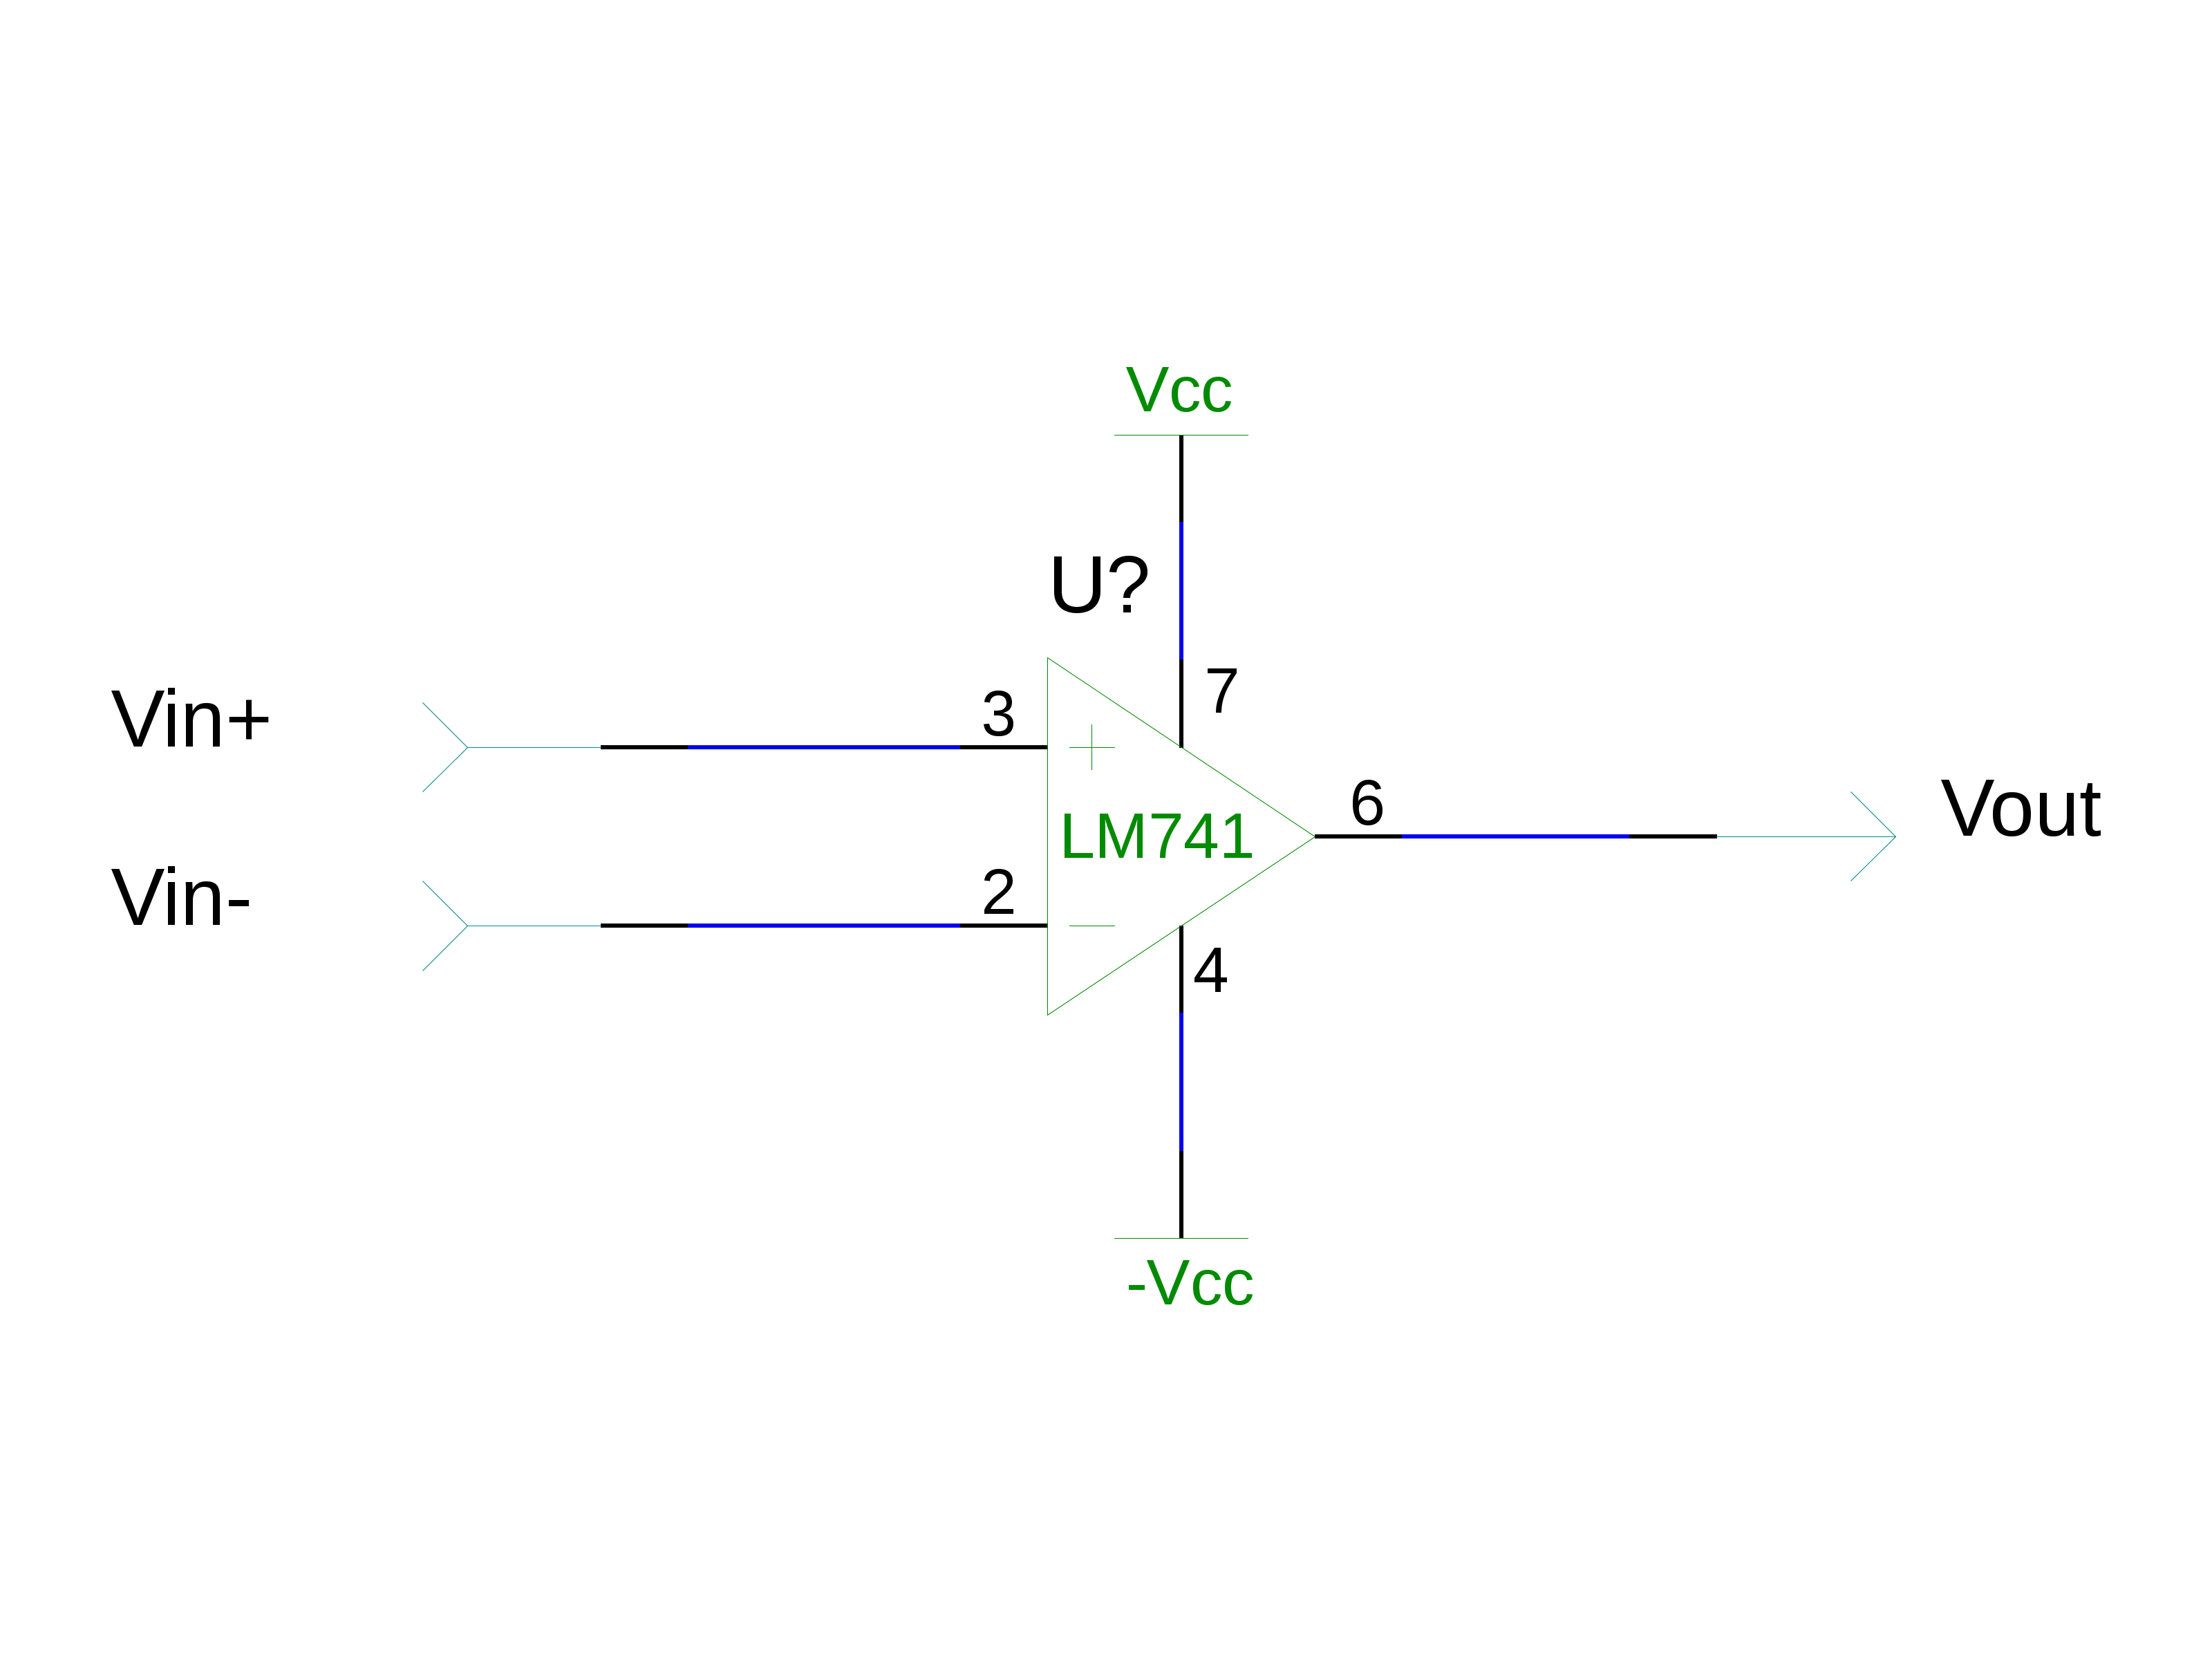
\includegraphics[width=\textwidth]{./images/comparator.png}
	\caption{A comparator circuit}
	\label{fig:comparator}
\end{figure}

\begin{enumerate}
\item Construct the comparator circuit
\item Set the inverting input to 0V using a potential divider
\item \label{enum:des:comp:probeout} Connect the oscilloscope probe to the output of the op-amp
\item Use the potentiometer provided to vary the input of the non-inverting input
\item \label{enum:des:comp:observe} Observe how the output changes
\item Set the inverting input to 7.5V using a potential divider
\item Repeat steps \ref{enum:des:comp:probeout} through \ref{enum:des:comp:observe}
\item Set the inverting input to -7.5V using a potential divider
\item Repeat steps \ref{enum:des:comp:probeout} through \ref{enum:des:comp:observe}
\item What difference would it make if you fixed the value of the non-inverting input with the potential divider, and varied the inverting input with the potentiometer?
\item Check if you're correct
\end{enumerate}

\subsubsection{Schmitt Trigger}
The schmitt trigger is an interesting design, as the input signal rises it will give a positive output, however in order to give a negative output the input needs to go significantly lower.

The circuit for this is shown below:

\begin{figure}[H]
	\centering
	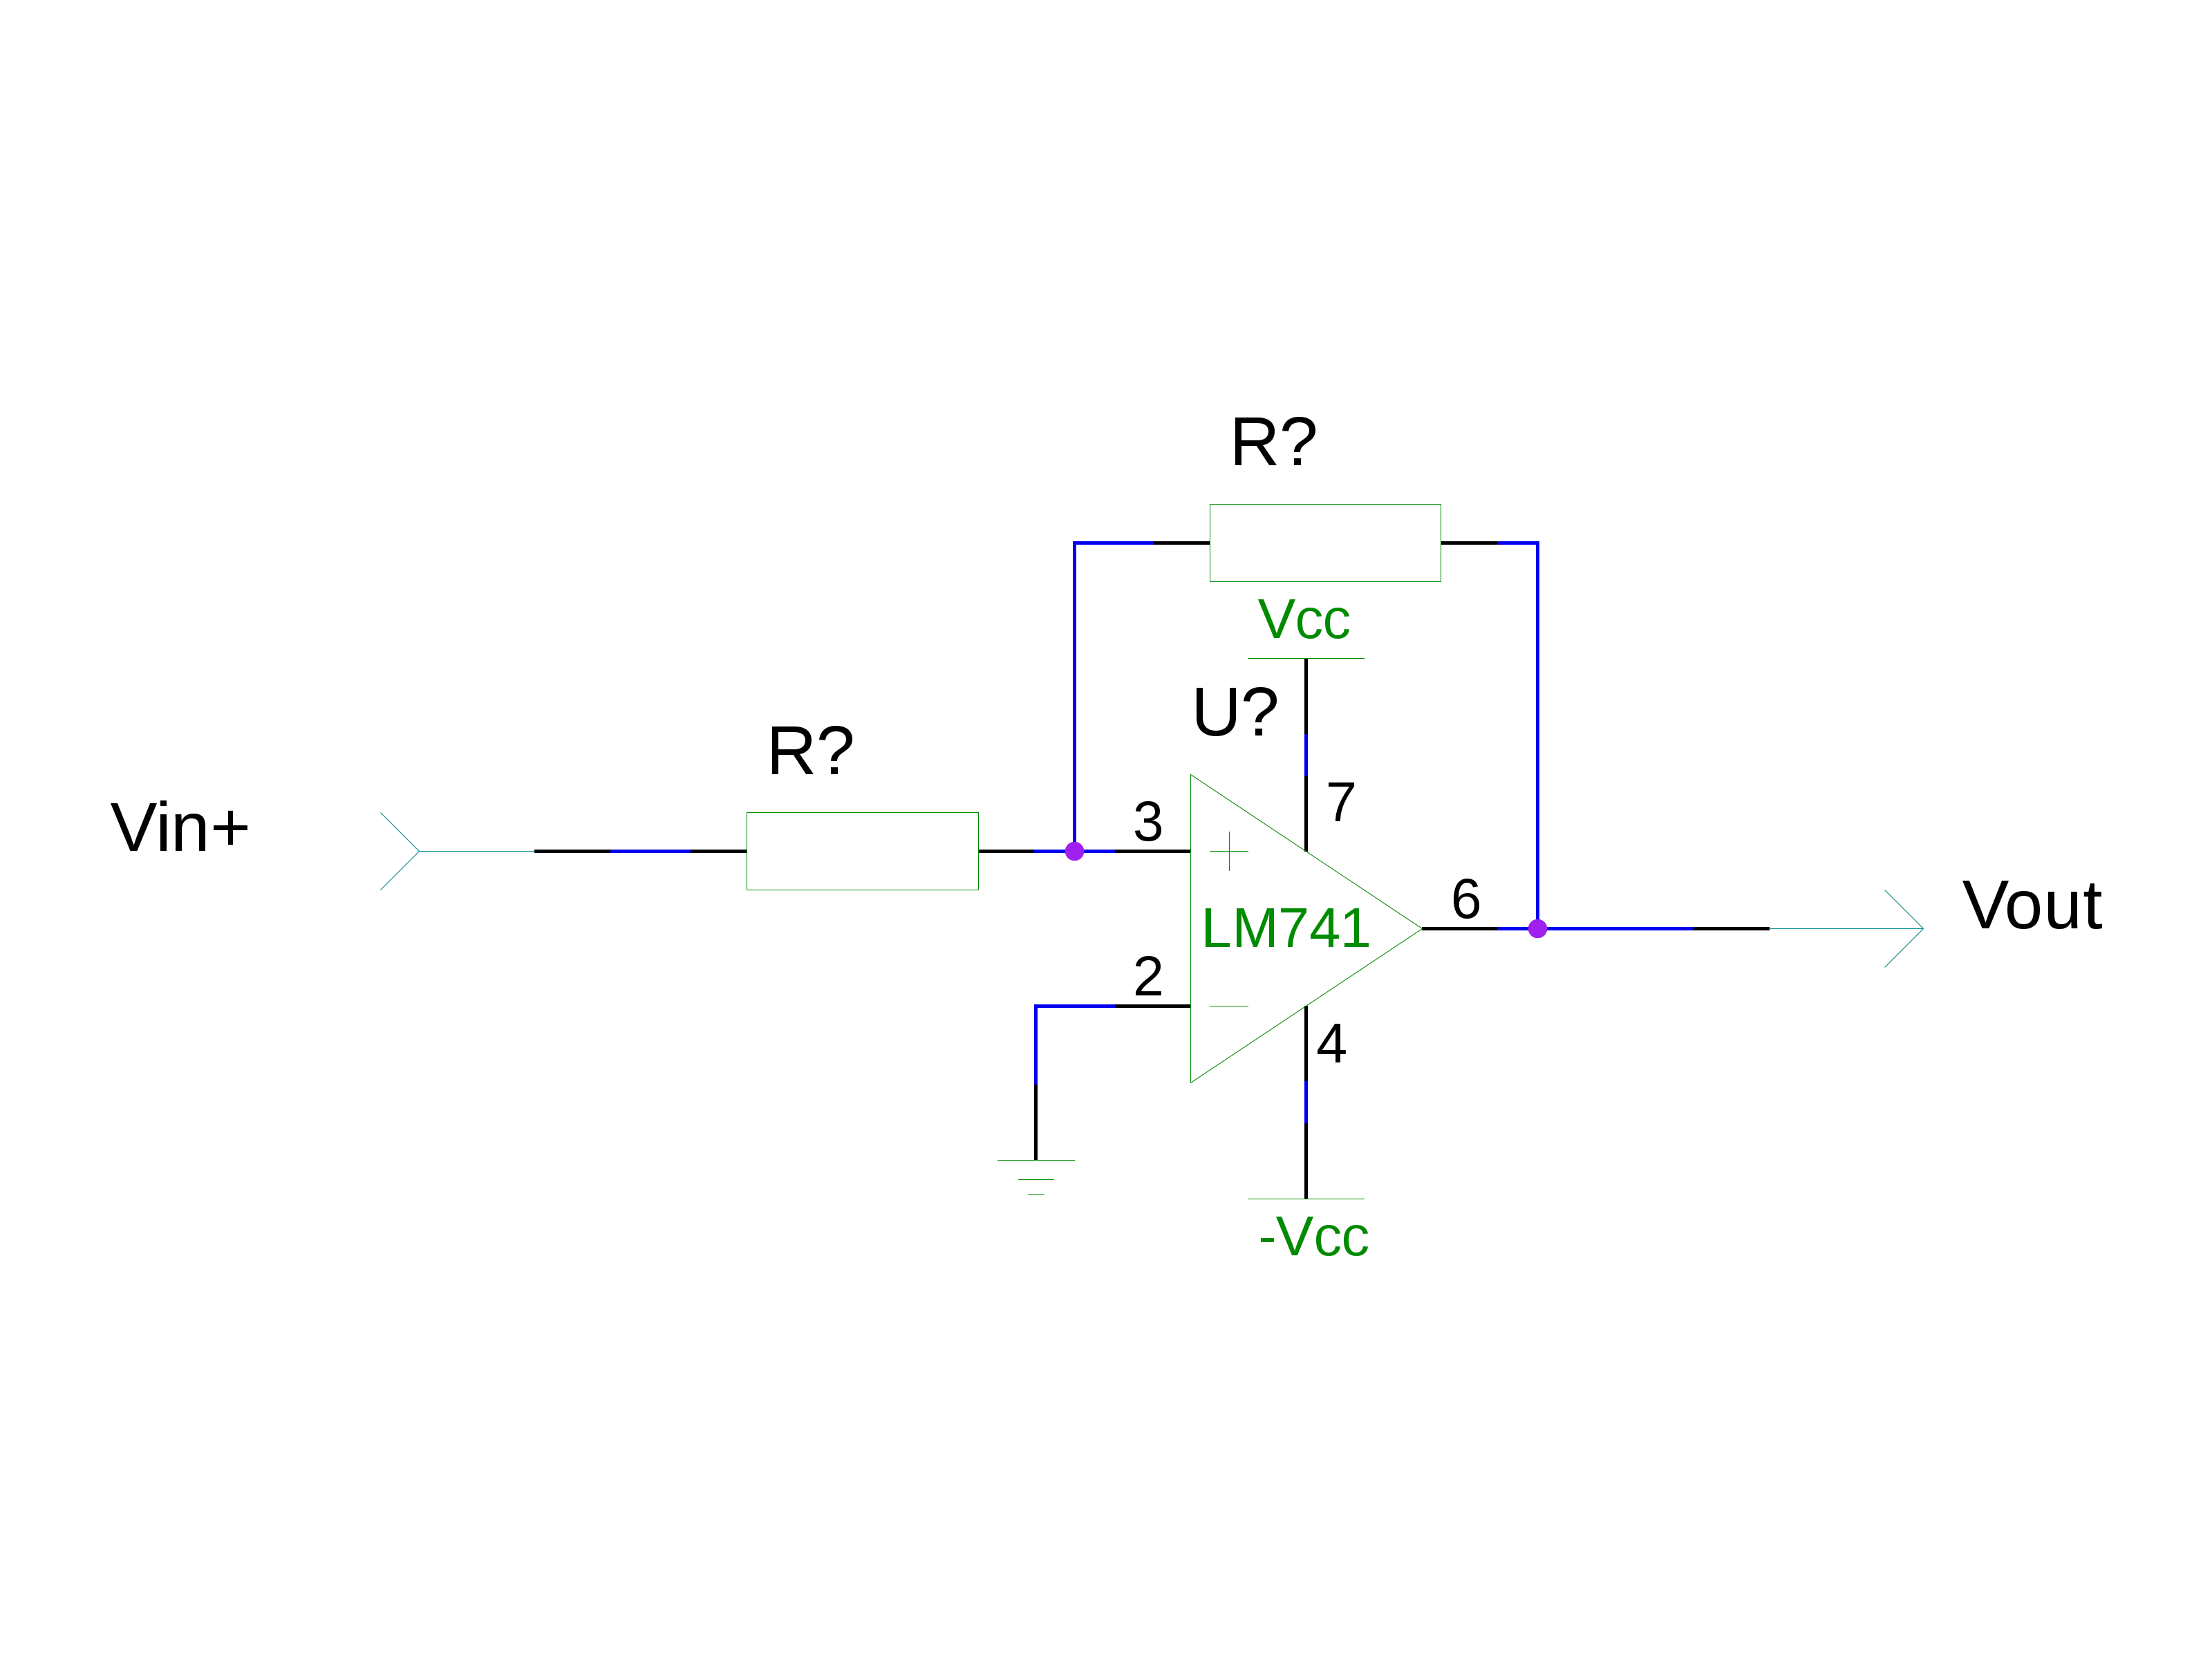
\includegraphics[width=\textwidth]{./images/schmitt.png}
	\caption{A Schmitt Trigger circuit}
	\label{fig:schmitt}
\end{figure}

\begin{enumerate}
\item Construct the schmitt trigger circuit, use R1 = $10K\Omega$ and R2 = $10K\Omega$
\item Connect the oscilloscope probe to the output of the schmitt trigger
\item \label{enum:des:schmitt:varyin} Vary the input between $\pm V_{cc}$ with the potentiometer
\item \label{enum:des:schmitt:observe} Observe the output
\item Set R1 = $5K\Omega$
\item Repeat steps \ref{enum:des:schmitt:varyin} through \ref{enum:des:schmitt:observe}
\item Set R1 = $20K\Omega$
\item Repeat steps \ref{enum:des:schmitt:varyin} through \ref{enum:des:schmitt:observe}
\item Set R1 = $10K\Omega$, R2 = $5K\Omega$
\item Repeat steps \ref{enum:des:schmitt:varyin} through \ref{enum:des:schmitt:observe}
\item Set R2 = $20K\Omega$
\item Repeat steps \ref{enum:des:schmitt:varyin} through \ref{enum:des:schmitt:observe}
\item Are there any similarities between any of the results?
\end{enumerate}

\subsubsection{Integrator}
The integrator gives an output which rises with a positive input.
With a negative input the output will fall, and with a zero input the output stays constant.

The circuit for this is shown below:

\begin{figure}[H]
	\centering
	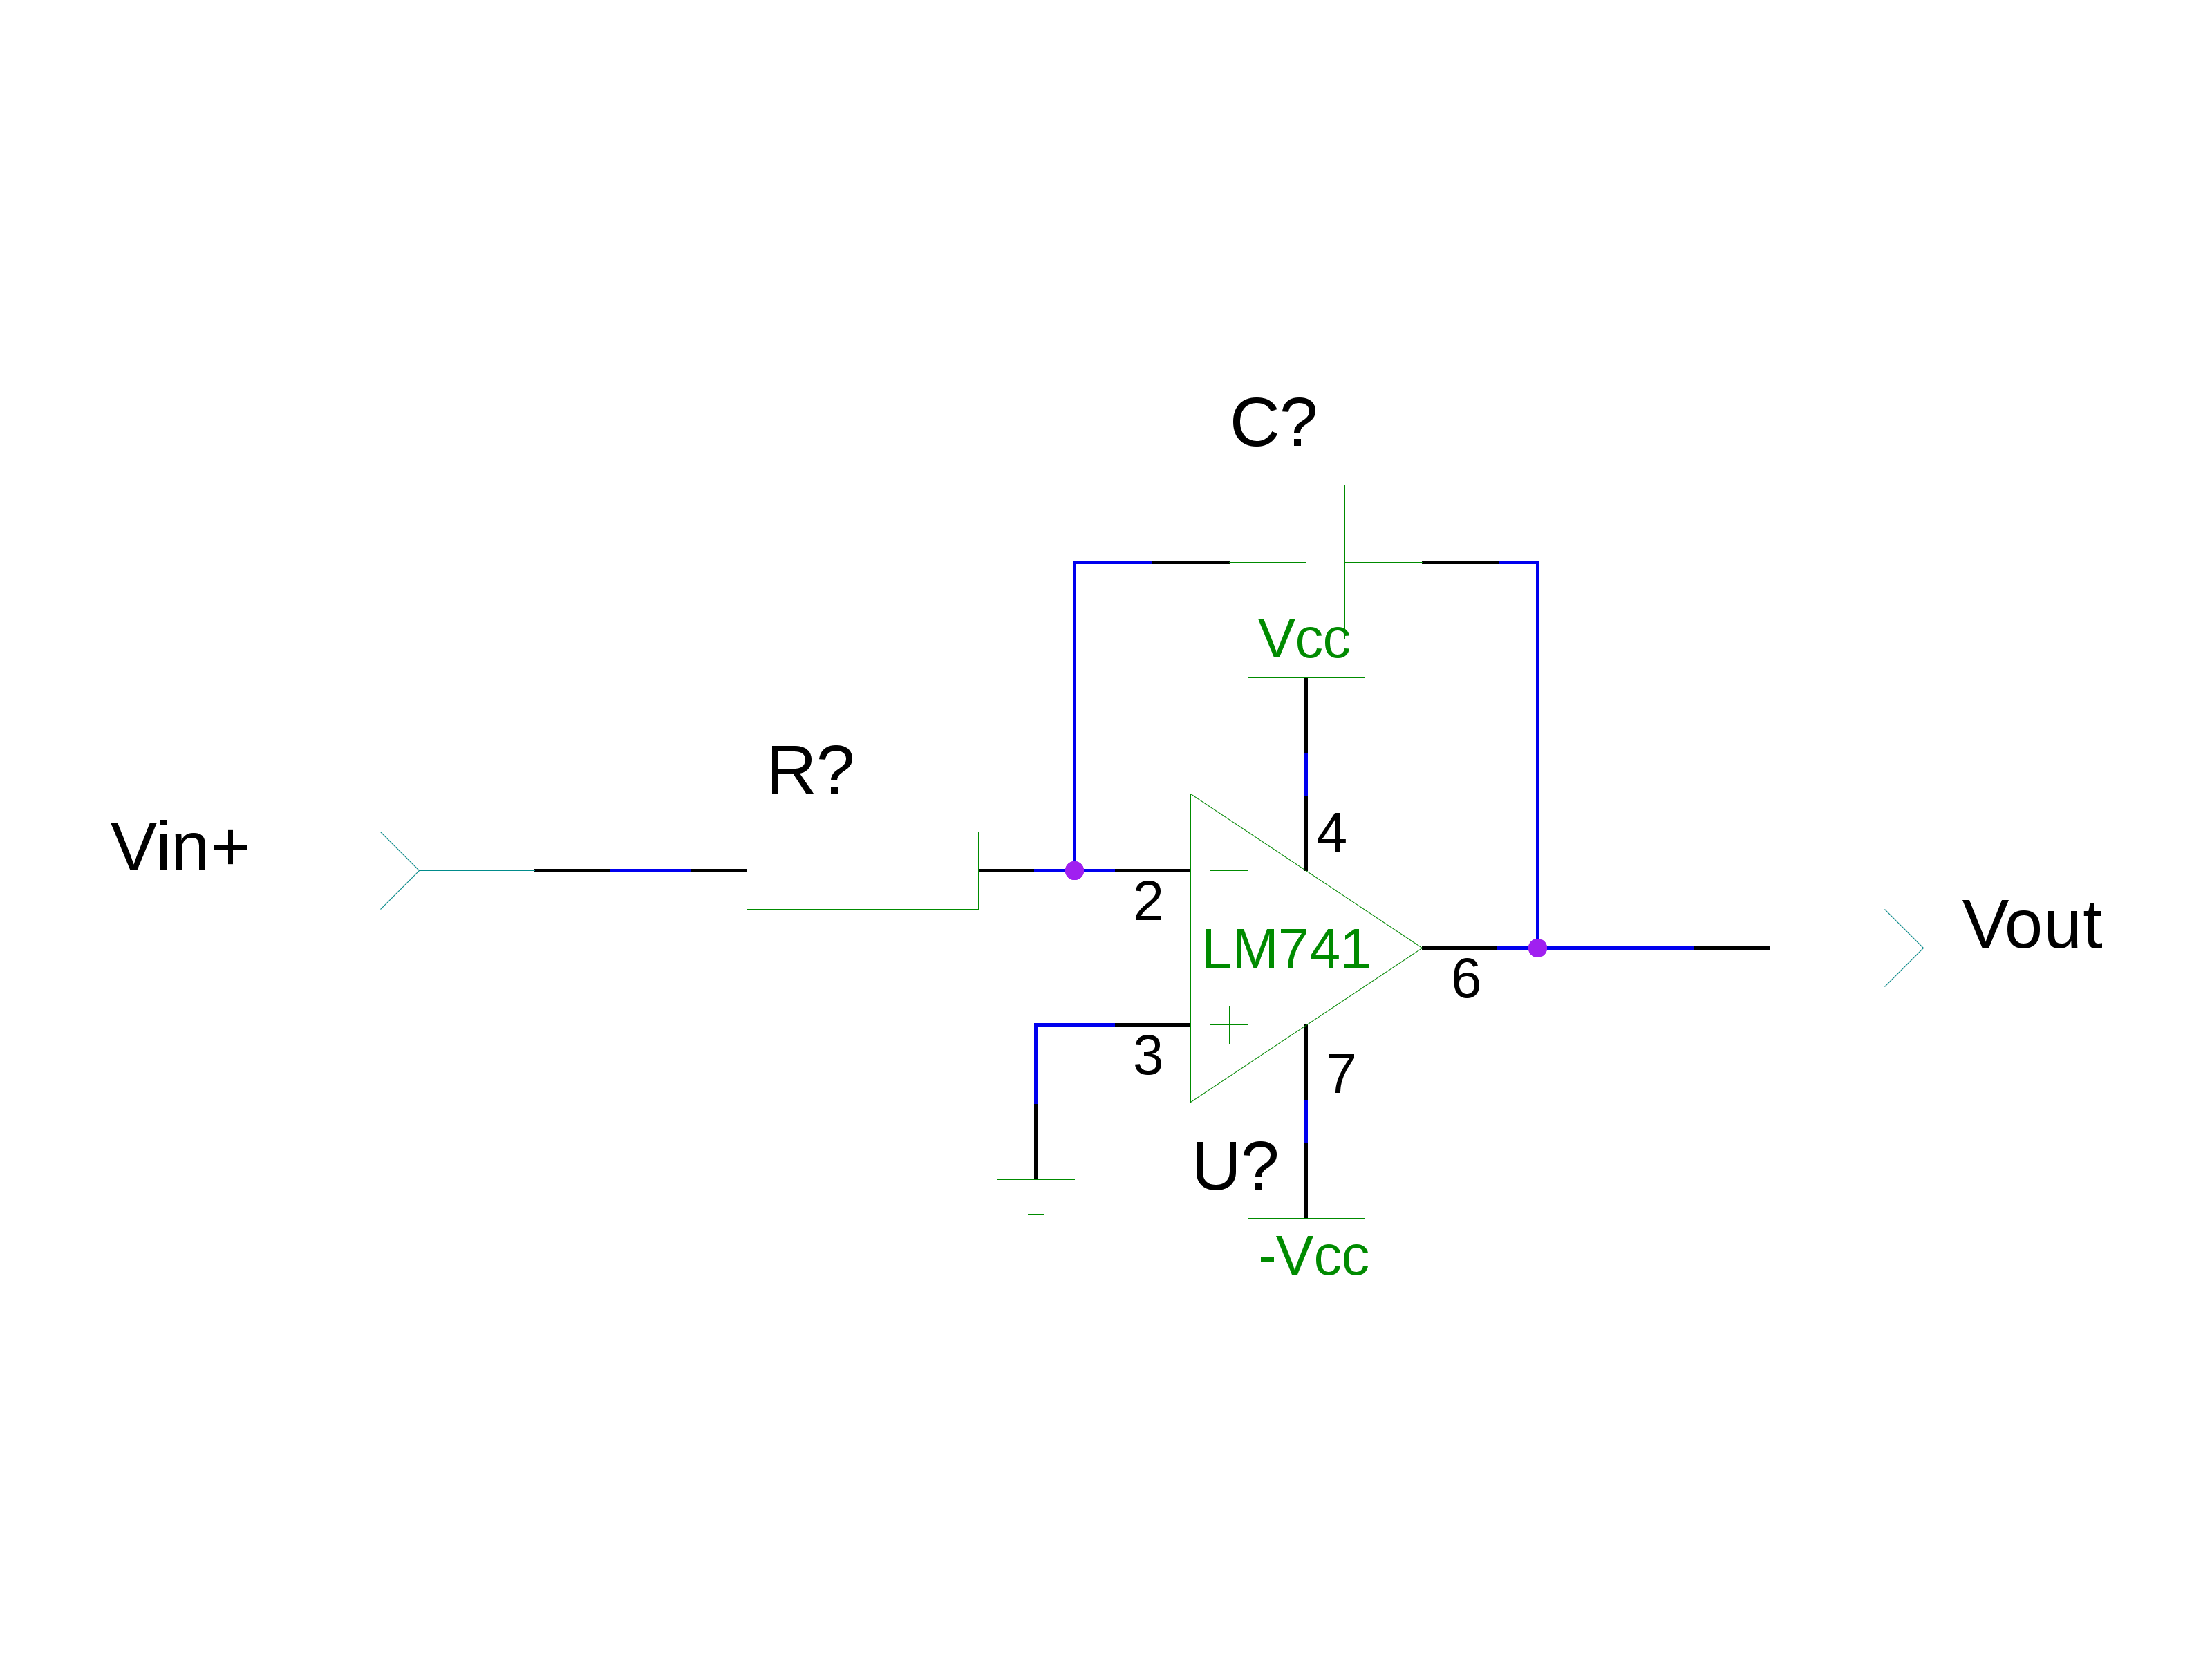
\includegraphics[width=\textwidth]{./images/integrator.png}
	\caption{An integrator circuit}
	\label{fig:integrator}
\end{figure}

\begin{enumerate}
\item Construct the integrator circuit, use R1 = $10K\Omega$, C1 = $20pF$
\item Connect the oscilloscope probe to the output
\item \label{enum:des:integrator:set0} Set the input of the circuit to 0V using the potentiometer
\item Turn on the power supplies
\item Use the potentiometer to vary the input between $\pm V_{cc}$
\item \label{enum:des:integrator:observe} Observe the output
\item Set R1 = $5k\Omega$
\item Repeat steps \ref{enum:des:integrator:set0} through \ref{enum:des:integrator:observe}
\item Set R1 = $20k\Omega$
\item Repeat steps \ref{enum:des:integrator:set0} through \ref{enum:des:integrator:observe}
\item Set R1 = $10k\Omega$, C1 = $10pF$
\item Repeat steps \ref{enum:des:integrator:set0} through \ref{enum:des:integrator:observe}
\item Set C1 = $40pF$
\item Repeat steps \ref{enum:des:integrator:set0} through \ref{enum:des:integrator:observe}
\item Are there any similarities between any of the results?
\end{enumerate}

\subsection{Microcontroller}
To demonstrate the use of a microcontroller the device has been preprogrammed to do a multiplication and display the output on two 7 segment displays.

\begin{enumerate}
\item Using the wire available, connect the outputs up to the 7 segment displays as shown in figure \ref{}
\item Connect pin ? to $GND$
\item \label{enum:des:uc:setGND} Connect pin ? to $GND$
\item Connect wires between the pins and and either $V_{cc}$ or $GND$ to create numbers as inputs
\begin{itemize}
\item Pins ?-? form input A, and are shown on the first 7 segment display
\item Pins ?-? form input B, and are shown on the second 7 segment display
\end{itemize}
\item \label{enum:des:uc:showout} Connect pin ? to $V_{cc}$, the two 7 segment displays now show a 2 digit number which is the result of $A \times B$
\item Repeat steps \ref{enum:des:uc:setGND} through \ref{enum:des:uc:showout} to confirm it operates as expected
\end{enumerate}
